\chapter{Примеры полученных графиков} \label{chapt3}

Ввод: из диапазона

Функция: $f (x, y) = x+y+1$

Режим: график

Длина регистра: $2^6$

Отображение: Монна

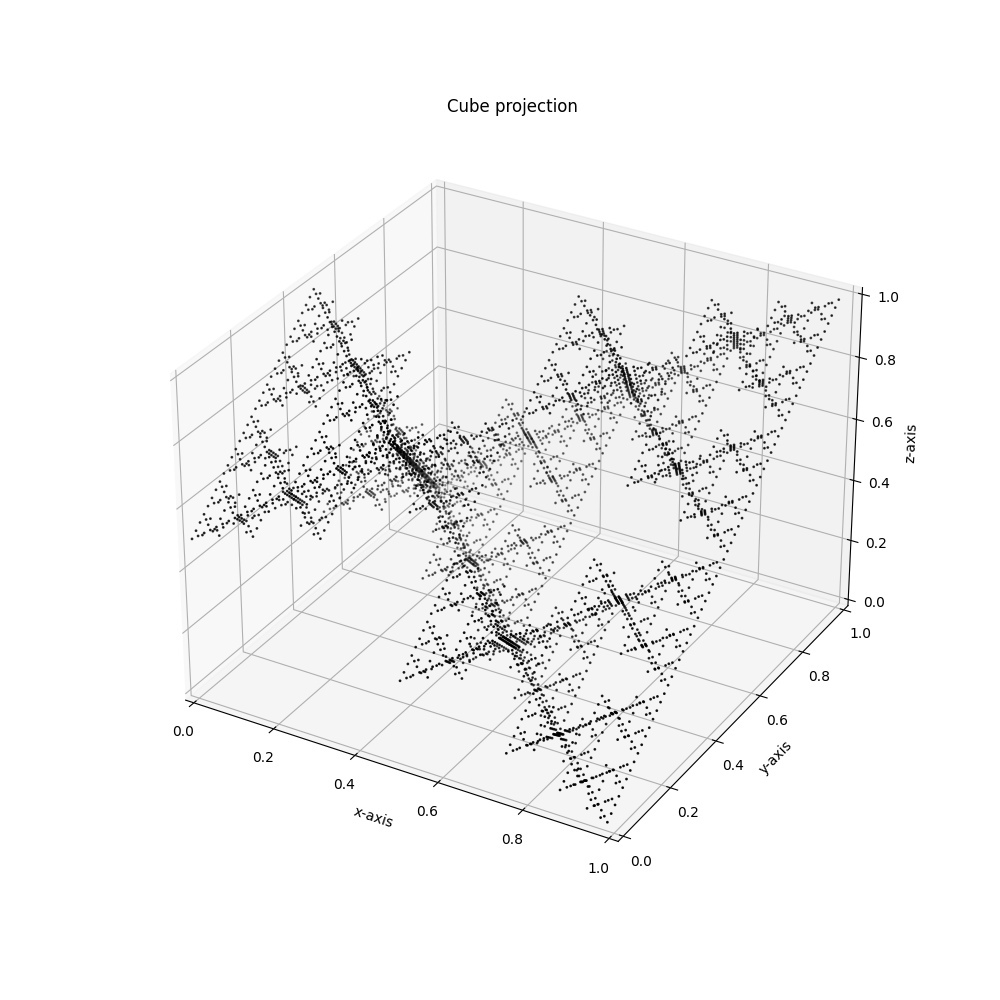
\includegraphics[scale=0.43]{gr1.jpg}

\newpage

Функция: $f(x, y) = x^3+y^2-(x*y \quad XOR \quad 17)$

Режим: график

Длина регистра: $2^6$

Отображение: Монна

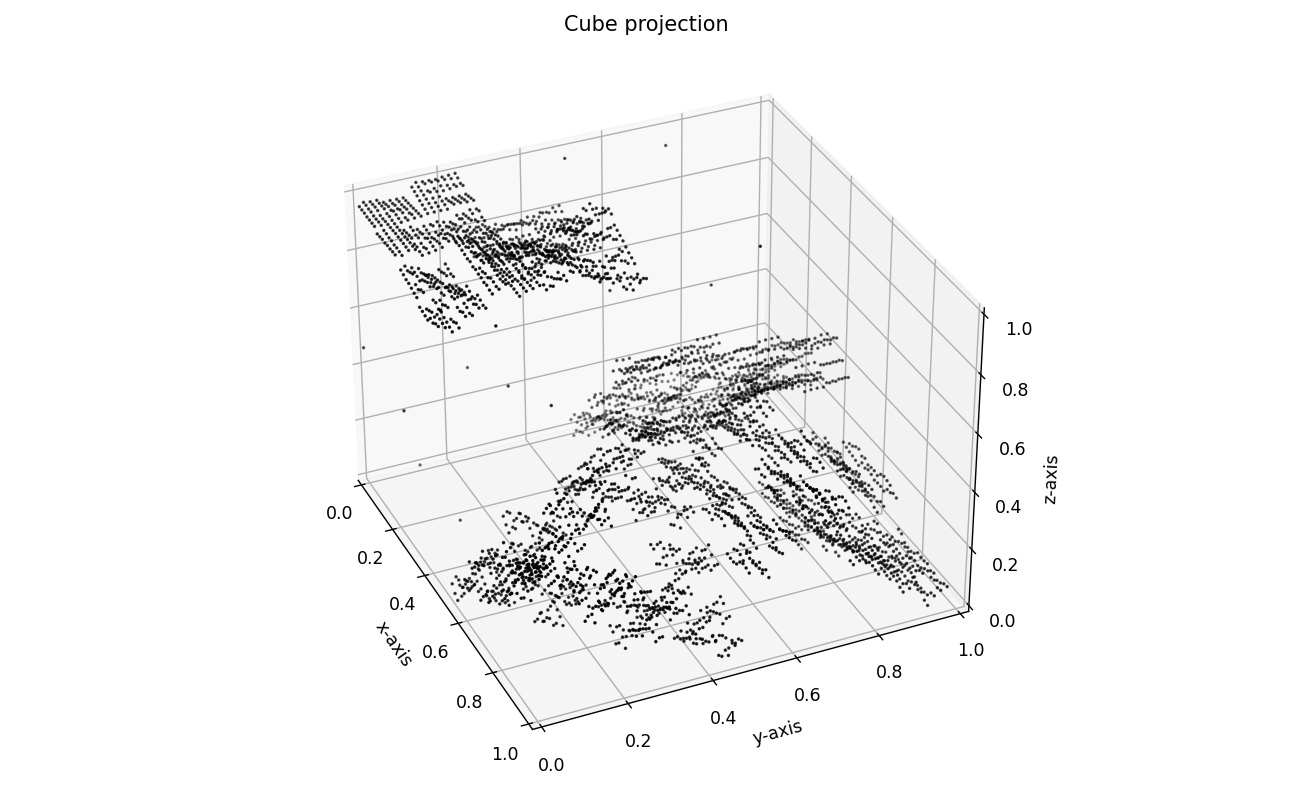
\includegraphics[scale=0.43]{gr2.jpg}

\newpage

Функция: $f(x, y) = (x^2 \quad XOR \quad y^2)+(x^2 \quad OR \quad y)$

Режим: график

Длина регистра: $2^6$

Отображение: Монна

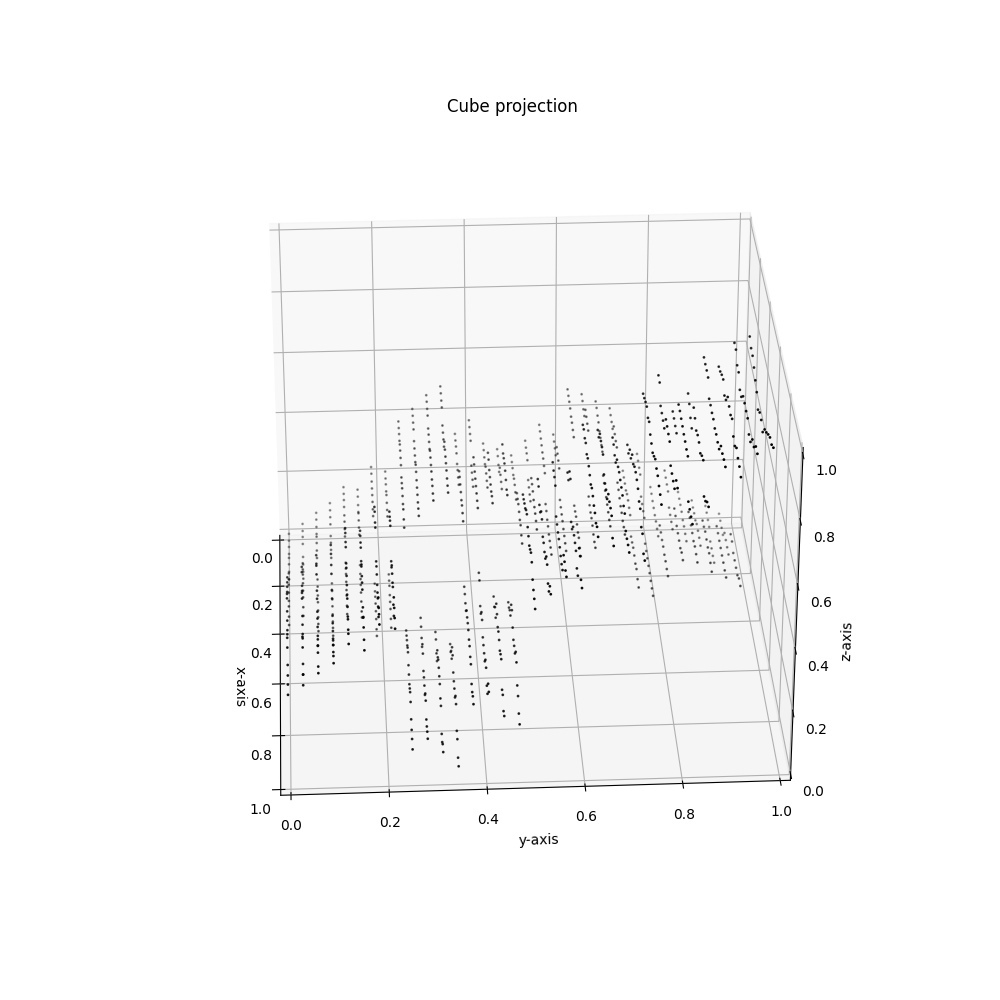
\includegraphics[scale=0.43]{gr_4.jpg}

\newpage

Функция: $f(x, y) = x+1$

Режим: график

Длина регистра: $2^{16}$

Отображение: Монна

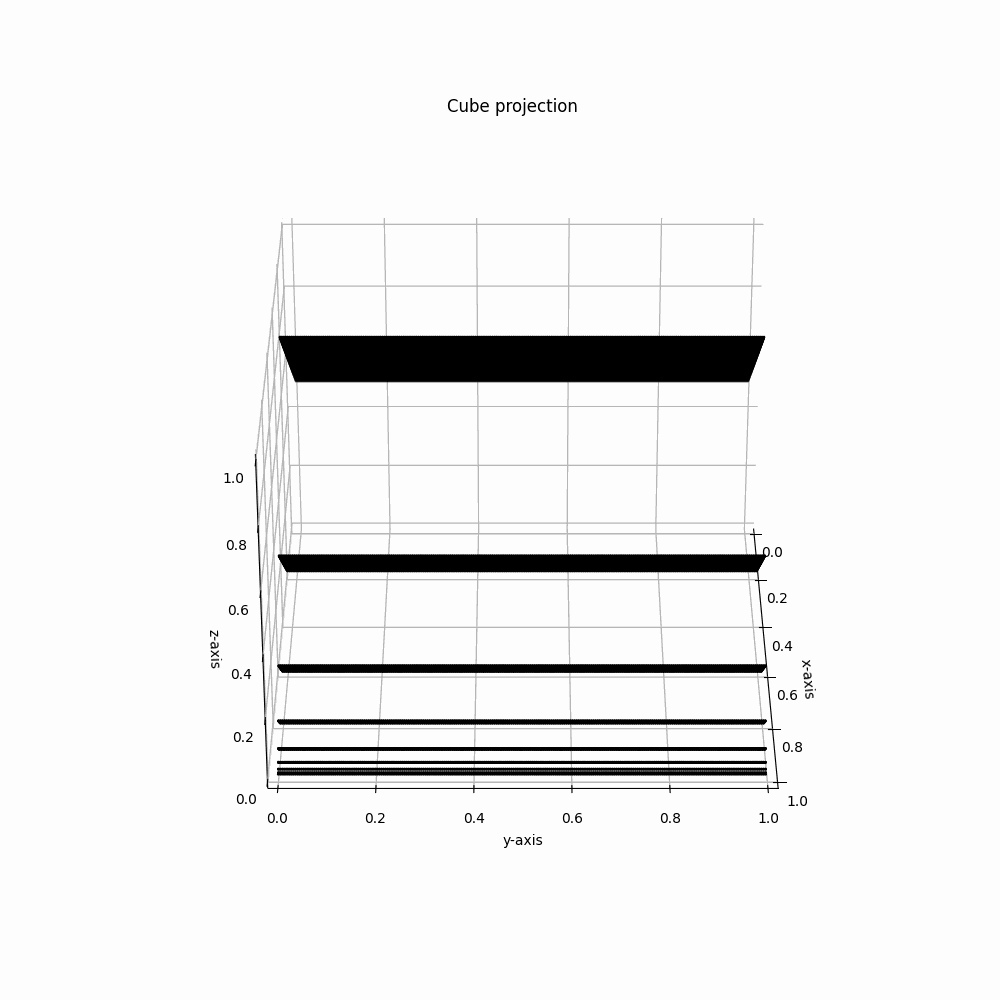
\includegraphics[scale=0.28]{gr_5.jpg}

Функция: $f(x, y) = y+1$

Режим: график

Длина регистра: $2^5$

Отображение: Монна

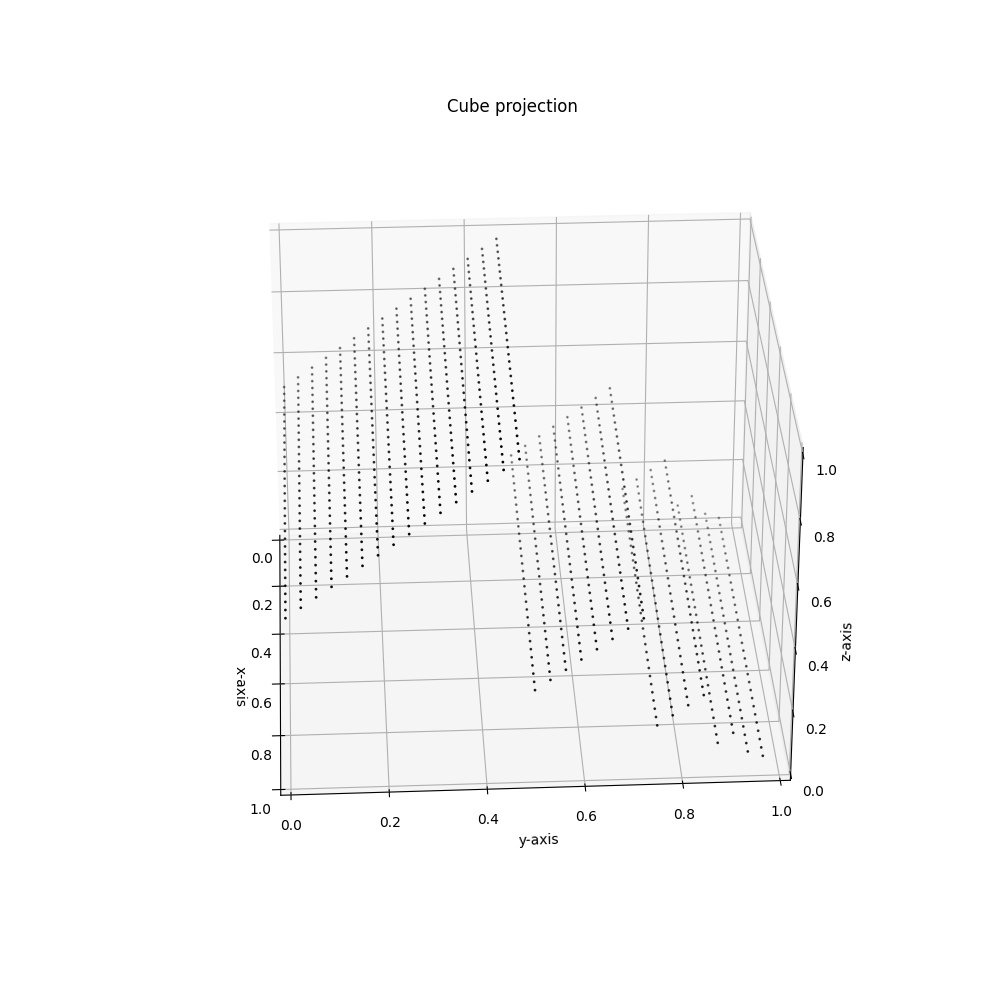
\includegraphics[scale=0.28]{gr_6.jpg}









\if 0
\newpage

Функция: $f (x, y) = x*y$

Режим: последовательность

Начальные значения: $x_0 = 13$ , 
$y_0 = 23$

длина регистра: $2^{63}$

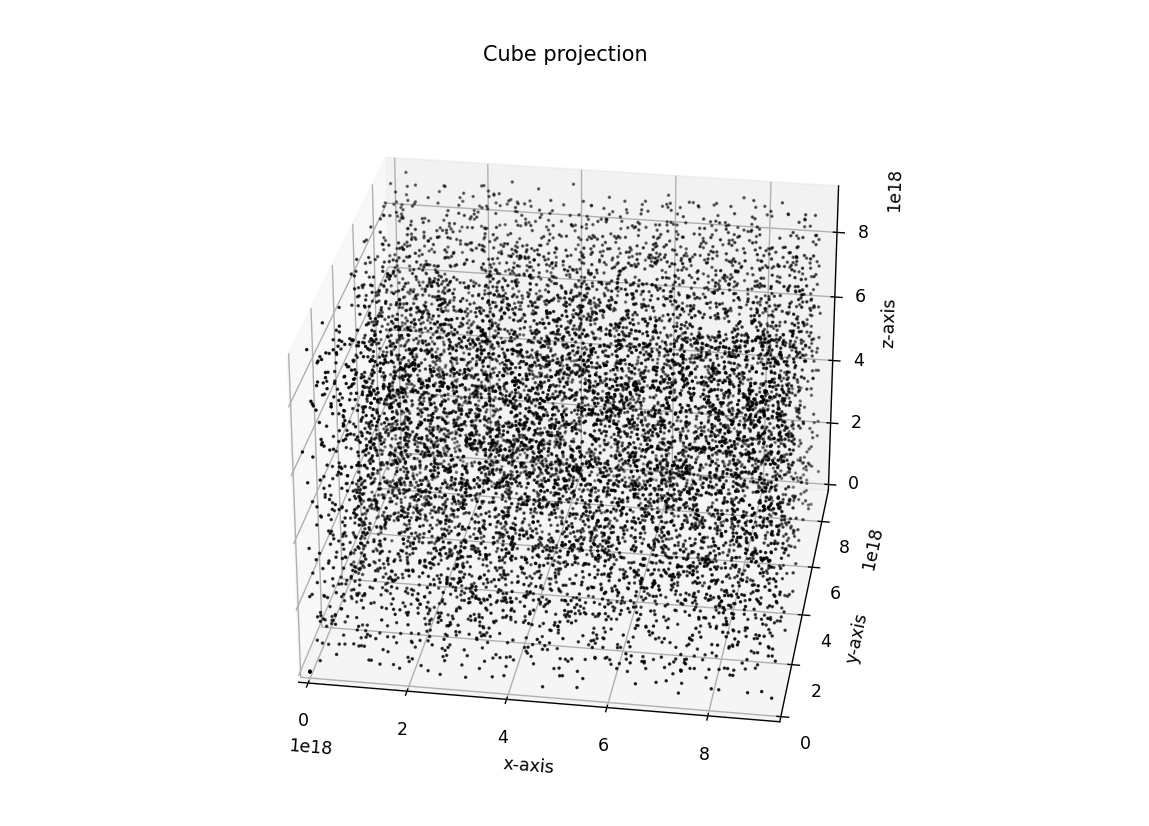
\includegraphics[scale=0.43]{gr3.jpg}

\fi 

\clearpage

